%! Author = joels
%! Date = 07/01/2022

% Sie können ...
% das Wesen der Softwarearchitektur beschreiben.
% den Unterschied zwischen Architektur und Entwurf ausführen.
% die Ziele der Softwarearchitektur erläutern.
% die Softwarearchitektur mittels Template, UML Paket-, Komponenten und Verteilungsdiagramm sowie mit NoUML-Zeichnungen problemadäquat dokumentieren.
% die wichtigsten Werkzeuge benennen.

\section{Einführung Softwarearchitektur}
\subsection{Was ist Softwarearchitektur?}
Definiert die grundlegenden \textbf{Prinzipien und Regeln} für die Organisation eines Systems sowie dessen \textbf{Strukturierung in Bausteinen und Schnittstellen} und deren Beziehungen zueinander wie auch zur Umgebung. $\rightarrow$ Beschreibt grobgranulare Strukturen wie: Komponenten mit Schnittstellen, Assoziationen/Interaktionen, Prinzipien \& Muster (Pattern)

\subsubsection{Bausteine}
Beschreiben statische Struktur des Systems. Bestehen aus:
\begin{itemize}[topsep=0pt, leftmargin=3mm]
    \setlength\itemsep{-0.3em}
    \item Pakete: Fassen untergeordnete Pakete bzw. Komponenten zu einer Einheit zusammen
    \item Komponenten: Klar definiertes Verhalten. Können Schnittstellen anbieten/konsumieren
\end{itemize}

\subsubsection{Architektur vs Entwurf (Design)}
\textbf{Architektur:}
\begin{itemize}[topsep=0pt, leftmargin=3mm]
    \setlength\itemsep{-0.3em}
    \item Legt grundlegende Strukturen fest
    \SubItem Bsp.: Mobile Native-App mit REST-Zugriff auf Web-Server
    \item Darstellung oft mit UML Komponentendiagramm
\end{itemize}
\textbf{Entwurf:}
\begin{itemize}[topsep=0pt, leftmargin=3mm]
    \setlength\itemsep{-0.3em}
    \item Legt feingranulare Struktur fest
    \SubItem Bsp.: Aufbau der Native-App: GUI – Funktionsebenen – Zugriff auf Server
    \item Darstellung oft mit UML-Klassendiagramm
\end{itemize}

\subsubsection{Rolle von Softwarearchitekt}
Arbeitet eng mit dem Requirements Engineering zusammen (Schwerpunkt auf NFA). Ist verantwortlich für:
\begin{itemize}[topsep=0pt, leftmargin=3mm]
    \setlength\itemsep{-0.3em}
    \item Grobgranularen Strukturen
    \item Querschnittskonzepte (z.B. Persistenz, Kommunikation, GUI)
    \item Erkennen/Aufzeigen von Konsequenzen bei Architekturentscheidungen
\end{itemize}
$\rightarrow$ Erarbeitet/bearbeitet die Technical User Stories des Product-Backlog

\subsection{Ziele von Softwarearchitektur}
Ziel der Softwarearchitektur ist die Sicherstellung einer adäquaten Softwareproduktequalität.
\begin{itemize}[topsep=0pt, leftmargin=3mm]
    \setlength\itemsep{-0.3em}
    \item Nützlichkeit: Applikation erfüllt ihre Funktion
    \item Festigkeit: Software ist stabil und langlebig
    \item Ästhetik: User Experience ist ansprechend
\end{itemize}

\subsubsection{ISO 25010 Softwareproduktequalitätsmodell}
\textbf{Benutzer:}
\begin{itemize}[topsep=0pt, leftmargin=3mm]
    \setlength\itemsep{-0.3em}
    \item Funktionalität
    \item Performanz und Effizienz
    \item Kompatibilität und Interoperabilität
    \item Benutzbarkeit
    \item Verfügbarkeit
\end{itemize}
\textbf{Betreiber \& Entwickler:}
\begin{itemize}[topsep=0pt, leftmargin=3mm]
    \setlength\itemsep{-0.3em}
    \item IT-Sicherheit
    \item Wartbarkeit
    \item Portierbarkeit
\end{itemize}


\subsection{Modellierung}
4 Sichten: Kontext, Baustein, Laufzeit und Verteilungssicht.
\subsubsection{Kontextsicht}
Das System steht im Zentrum als Black-Box. Alle Umsysteme und relevanten Stakeholder sind als externe Agenten dargestellt. Die Verbindungen von und zum System bilden Datenflüsse ab.\\
\textbf{Diagramme:} Kontext- oder UML-Diagramm

\subsubsection{Bausteinsicht}
Struktureller Aufbau des Systems\\
\textbf{Paketdiagramm:}\\
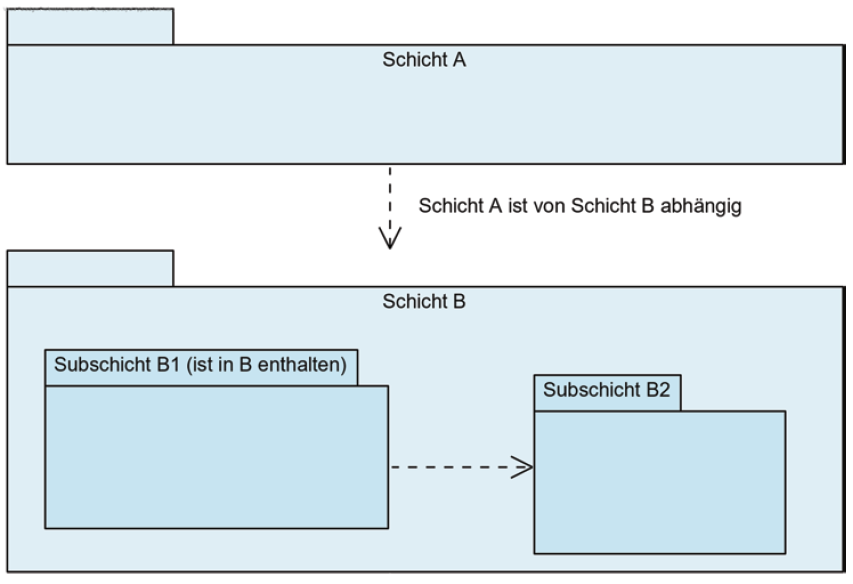
\includegraphics[width=\linewidth]{paketdiagramm}
\textbf{Komponentendiagramm:}\\
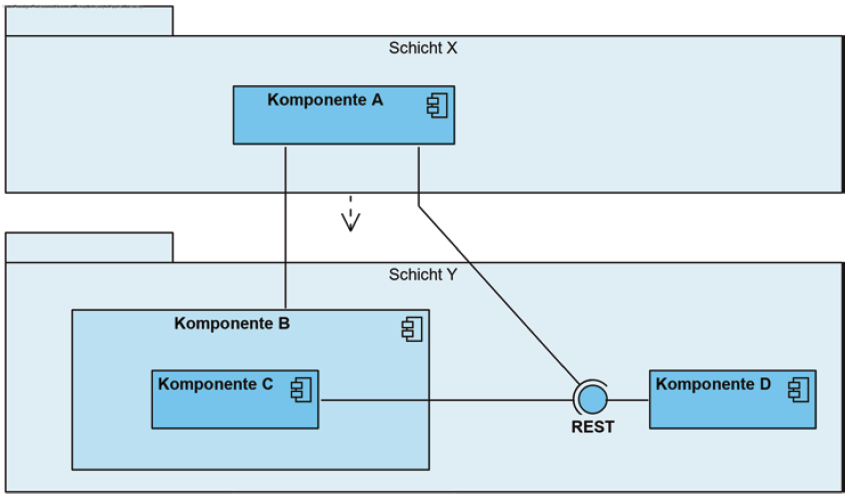
\includegraphics[width=\linewidth]{komponentendiagramm}

\subsubsection{Laufzeitsicht}
Fokussiert auf die dynamischen Aspekte wie Prozessabläufe, Interaktionen zwischen Bausteinen und Verhalten.\\
\textbf{Diagramme:} Sequenz-, Aktivitäts- und Zustands-Diagramm

\subsubsection{Verteilungssicht}
\textbf{Darstellen:} Komponenten, welche in einer spezifischen Laufzeitumgebung installiert werden.\\
\textbf{Diagramm:} Deploymentdiagramm

\subsubsection{Werkzeuge}
\textbf{Textbasierte Dokumentation:} Wiki für kollaborales Erarbeiten der Inhalte, plus Versionierung. Bsp: Confluence\\
\textbf{Modellierungswerkzeuge:} Unterstützung von Diagrammsprachen wie UML, SysMl. Bsp: Visual Paradigm\\
\textbf{Code-Analysetool:} Statische Analyse und Bewertung der technischen Qualität von Sourcecode. Bsp: SonarQube\\
\textbf{Testtools:}

